\chapter{Desarrollo de la solución}
\textit{``El desarrollo de aplicaciones móviles resulta desafiante por la gran variedad de dispositivos
móviles con diferentes sistemas operativos, características y tamaños'' \cite{7021823}. Esta tarea
la suplementa Flutter con sus widgets, permitiendo
desarrollar todo tipo de vistas con un diseño adaptativo para la mayoría de dispositivos.
}

\section{Prototipado de pantallas}
El diseño de la totalidad de pantallas se ha realizado siguiendo las pautas y directrices marcadas por
el estándar \textit{Material Design}. Su gran contenido de iconos, estilos y componentes se ha plasmado,
gracias al paquete \textit{material}, directamente en el aplicativo.

Antes del desarrollo completo de cada una de las pantallas del aplicativo, se ha optado por el diseño de
\textit{MockUps}, indicando cada uno de los casos de uso y requisitos funcionales vistos en el Capítulo 
3, indicados por los identificadores del \textit{1 al 21}.

\begin{figure}[H]
    \centering
    \begin{subfigure}[b]{0.38\linewidth}
      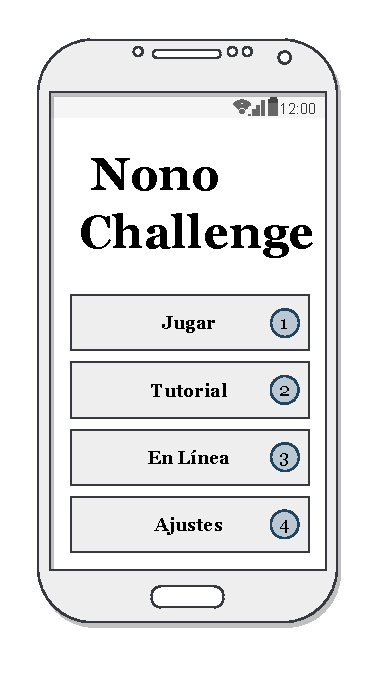
\includegraphics[width=\linewidth]{images/screen1.pdf}
    \end{subfigure}
    \begin{subfigure}[b]{0.38\linewidth}
      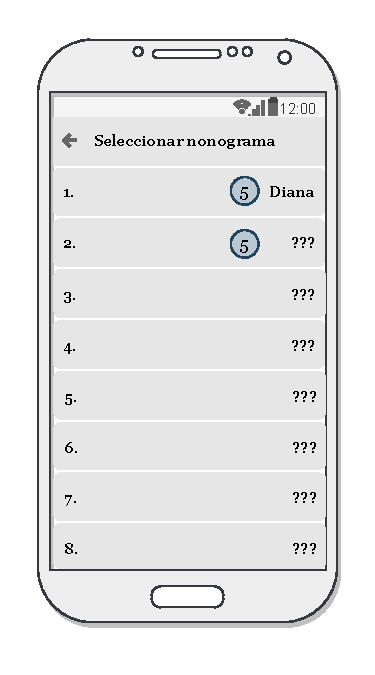
\includegraphics[width=\linewidth]{images/screen2.pdf}
    \end{subfigure}
    \caption{MockUps Pantalla de Inicio y Selector de niveles clásicos}
    \label{fig:design-1}
\end{figure}

La Pantalla de Inicio será la encargada de proveer al usuario el acceso de todos los casos
de uso y requisitos funcionales disponibles.

La pantalla de Selector de niveles clásicos mostrará todos los niveles disponibles predeterminados del sistema,
muchos de ellos extraídos de los libros \textit{Griddlers}, publicados por el noticiero británico 
\textit{Sunday Telegraph}.
A medida los niveles han sido superados se descubrirá el nombre de la figura que representa,  \autoref{fig:design-1}.

\begin{figure}[H]
    \centering
    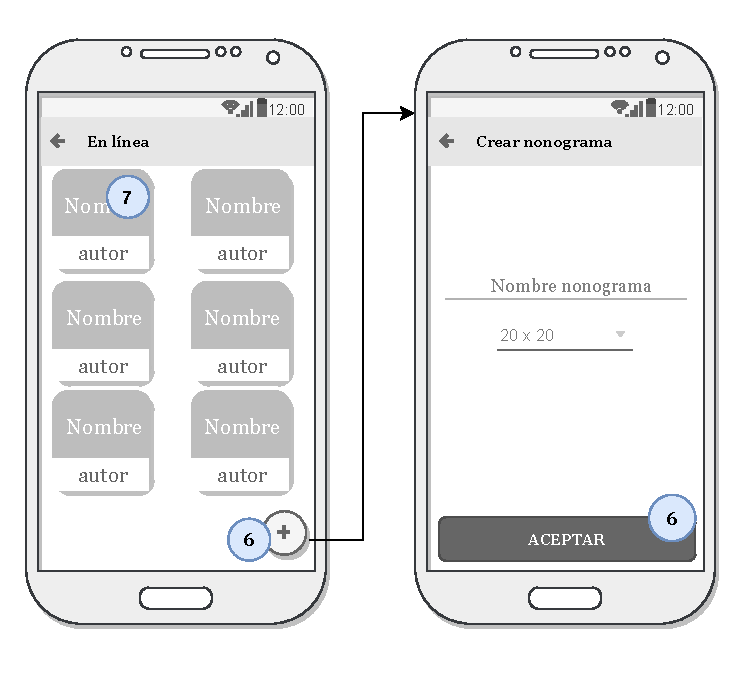
\includegraphics[scale=0.83]{images/screen3.pdf}
    \caption{MockUps Pantalla de niveles online y publicación de nonogramas}
    \label{fig:design-2}
\end{figure}

\begin{figure}[H]
  \centering
  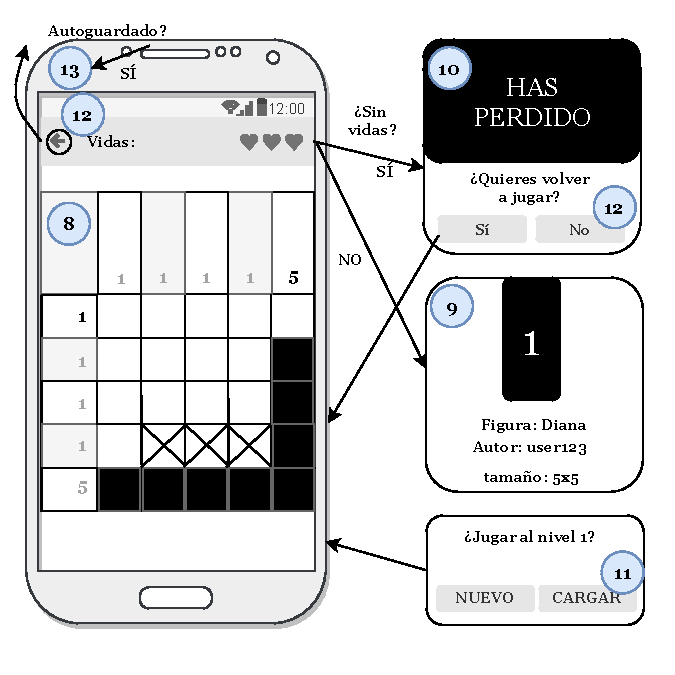
\includegraphics[scale=0.83]{images/screen4.pdf}
  \caption{MockUp Pantalla de resolución de nivel}
  \label{fig:design-3}
\end{figure}

En la  \autoref{fig:design-3} se puede observar el diagrama de flujo de resolución
de nivel. 
Como se puede apreciar, la apariencia y esencia del rompecabezas es fiel al de los medios tradicionales:

\begin{itemize}
  \item[$\bullet$] Las celdas pintadas representan las celdas que se han seleccionado (con un clic) y
  resultan correctas
  \item[$\bullet$] Aquellas celdas con \textit{equis} son las marcadas  por el
  usuario (con doble clic sobre ella), asegurando que no son correctas.
  \item[$\bullet$] Los bloques de los extremos contienen el número
  de celdas correctas de esa fila o columna, los cuales se van difuminado a medida que se van
  resolviendo por el usuario.
\end{itemize}

El jugador puede abandonar el nivel en cualquier momento, guardando su progreso si la opción de autoguardado
está activada. En el instante de resolverlo satisfactoriamente (con al menos una vida) se mostrarán
las características del mismo, y en el caso contrario, la opción de volver a intentarlo.

\begin{figure}[H]
  \centering
  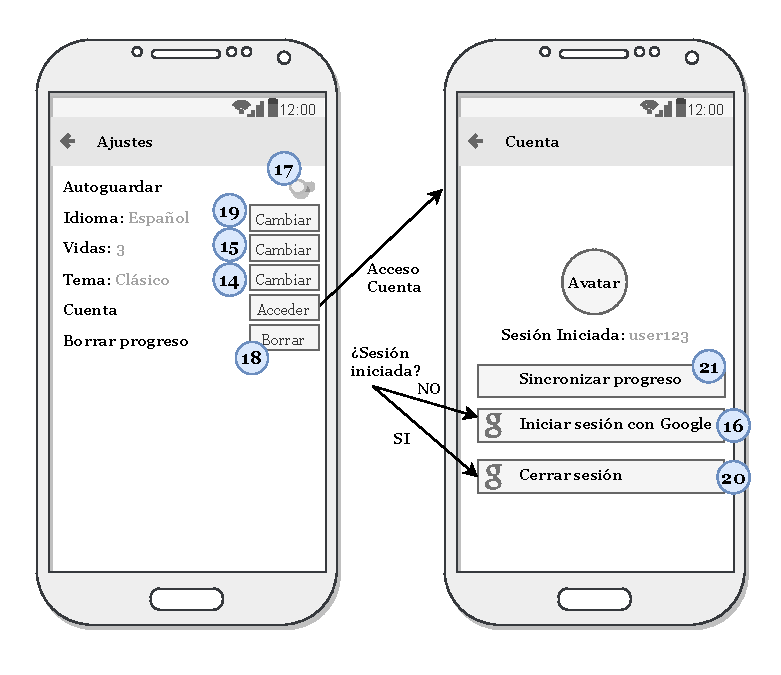
\includegraphics[scale=0.83]{images/screen5.pdf}
  \caption{MockUp Pantalla de ajustes y cuenta}
  \label{fig:design-4}
\end{figure}

En la pantalla se pueden configurar propiedades relativas a: 

\begin{itemize}
  \item[$\bullet$] La experiencia de juego como: la posibilidad de autoguardado y
  el número de vidas.
  \item[$\bullet$] El idioma de la totalidad del sistema, por ahora para este \textit{MVP}, entre español e inglés.
  \item[$\bullet$] La combinación de colores que componen el tema del aplicativo.
\end{itemize}

El usuario puede borrar el progreso de todos sus niveles jugados mediante la opción de borrar
progreso, además de sincronizarlo con el \textit{servicio en nube} desde el apartado cuenta, 
iniciando sesión previamente (\autoref{fig:design-4})

\section{Estructura del proyecto}
Es importante que en un desarrollo de software se establezca una estructura propia de la arquitectura elegida,
para mantener una modularidad y escalabilidad a nivel de sistema.
Para ello, siguiendo las directrices del modelo \textit{Clean Architecture}, se ha definido el siguiente
árbol de directorios:

\definecolor{folderbg}{RGB}{230,230,230}
\definecolor{folderborder}{RGB}{110,144,169}

\def\Size{4pt}
\tikzset{
  folder/.pic={
    \filldraw[draw=folderborder,top color=folderbg!50,bottom color=folderbg]
      (-1.05*\Size,0.2\Size+5pt) rectangle ++(.75*\Size,-0.2\Size-5pt);  
    \filldraw[draw=folderborder,top color=folderbg!50,bottom color=folderbg]
      (-1.15*\Size,-\Size) rectangle (1.15*\Size,\Size);
  }
}
\begin{figure}[H]
\begin{center}
\begin{forest}
  for tree={
    font=\scriptsize\ttfamily,
    grow'=0,
    child anchor=west,
    parent anchor=south,
    anchor=west,
    calign=first,
    inner xsep=7pt,
    edge path={
      \noexpand\path [draw, \forestoption{edge}]
      (!u.south west) +(7.5pt,0) |- (.child anchor) pic {folder} \forestoption{edge label};
    },
    before typesetting nodes={
      if n=1
        {insert before={[,phantom]}}
        {}
    },
    fit=band,
    before computing xy={l=15pt},
  }  
[nonochallenge
  [assets ----imágenes{,} iconos{,} y fuentes.
  ]
  [lib ----código fuente dart.
    [api ----funciones y llamadas Firebase.
    ]
    [common ----archivos globales del sistema.
      [theme  ----temas del aplicativo.
      ]
      [utils  ----funciones de utilidad.
      ]
      [widgets  ----widgets comunes del sistema.
      ]
    ]
    [core ----clases genéricas de funcionalidad.
      [error ----clases error y excepciones.
      ]
      [platform ----detección de conexiones ej:internet.
      ]
      [usecase ----definición casos de uso.
      ]
    ]
    [di ----inyector de dependencias.
    ]
    [features ----funcionalidades del sistema.
      [feature1 ----funcionalidad.
        [data ----capa de datos.
          [datasources ---- comunicación con Firebase y base de datos local.
          ]
          [models ----implementación de las entities con serialización y funciones.
          ]
          [repositories\_impl ----implementación de los repositorios de dominio.
          ]
        ]
        [domain ----capa de dominio.
          [entities ----modelos de datos.
          ]
          [repositories ----definición genérica de repositorio.
          ]
          [usecases ----definición de los casos de uso de la funcionalidad.
          ]  
        ]
        [presentation ----capa de presentación y lógica.
          [bloc ----manejador de estados y capa de lógica.
          ]
          [pages ----pantallas de la característica.
          ]
          [widgets ----componentes que componen las pantallas.
          ]
        ]
      ]
      [... ----más funcionalidades.
      ]
    ]
    [i10n ----archivos de traducción.
    ]
  ]
  [tests ----tests del sistema
    [feature1 ----suites de test de funcionalidad: unitarios{,} lógica y widgets.
    ]
    [...
    ]
  ]
]
\end{forest}
\label{fig:tree-1}
\caption{Estructura de directorios de \textit{nonogramchallenge}}
\end{center}
\end{figure}

\section{Codificación del aplicativo}
El proceso de codificación se ha realizado posteriormente a la creación de una \textit{suite de tests} de funcionalidades, siguiendo las pautas y
reglas establecidas por la metodología TDD, proceso documentado en el sexto capítulo.

En el siguiente apartado se explicará el \textit{modus operandi} de la codificación de funcionalidades, acompañado de ejemplos definidos 
en el \autoref{cap:anexo2}, comenzando por la capa de presentación.

\subsection{Desarrollo de la capa de presentación}
La creación de cada una de las pantallas y sus componentes se ha realizado, como no podría ser de otra forma, a partir de un \textit{árbol de widgets}. 
Para el desarrollo de pantallas se ha optado por usar widgets inmutables, llamados, \textit{stateless}, en contraposición a los de tipo \textit{stateful},
con estado mutable. \cite{10.1007/978-981-15-1465-4_56} 

Esta práctica permitirá que la \textit{capa de presentación} contenga la mínima lógica posible, pudiendo en un futuro reutilizarla
en otras funcionalidades del sistema o incluso en otras soluciones.

\begin{figure}[H]
  \centering
  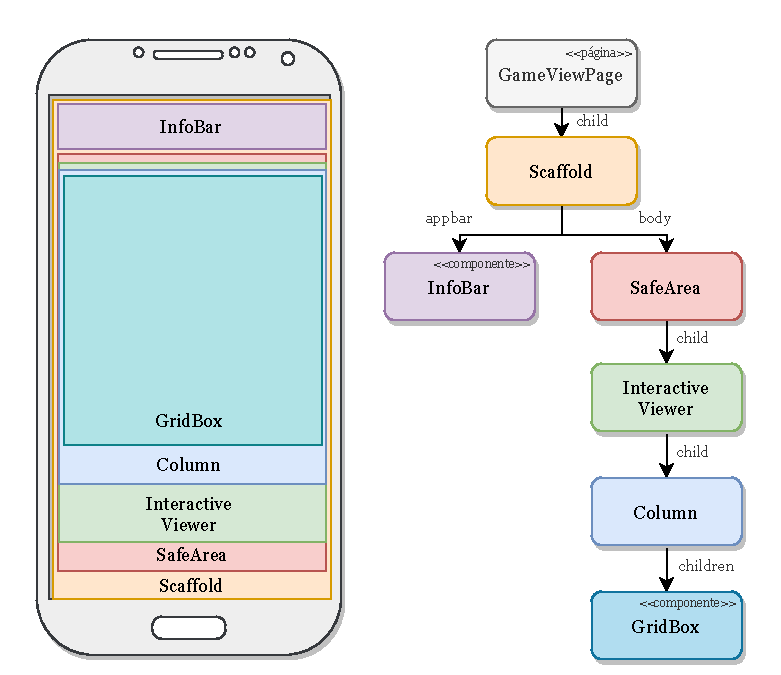
\includegraphics[scale=0.83]{images/treewidgets.pdf}
  \caption{Árbol de widgets Pantalla de Resolución de nivel}
  \label{fig:tree-widgets-1}
\end{figure}

En la \autoref{fig:tree-widgets-1} y \autoref{cap:anexo1-1} se puede visualizar el \textit{árbol de widgets} de la pantalla de resolución de nivel, los cuales
se ``construyen'' mediante el método \textit{build()}.

Esta vista contiene algunos widgets de interés que se han usado para mejorar la experiencia de usuario como:
\begin{itemize}
  \item[$\bullet$] \textit{SafeArea}: contenedor que acopla la pantalla en el caso que el dispositivo contenga elementos físicos como \textit{notch}, 
  statusbar, marcos de pantalla redondeados...
  \item[$\bullet$] \textit{InteractiveViewer}: permite al usuario realizar gestos como acercar, alejar y mover el rompecabezas 
  para casos en los que el \textit{nonograma} es de grandes dimensiones. 
\end{itemize}

\subsection{Desarrollo de la capa de lógica}
Para implementar la capa de lógica, se usará el paquete \textit{flutter\_bloc}, para ello se definirán todos los 
posibles estados y eventos presentes en dicha funcionalidad y una clase \textit{BLoC} que se encargue de 
``manejar'' el flujo de cambios de estado.

A continuación, se mostrará un diagrama de flujo de estados de la funcionalidad \textit{lista de nonogramas en línea}.

\begin{figure}[H]
  \centering
  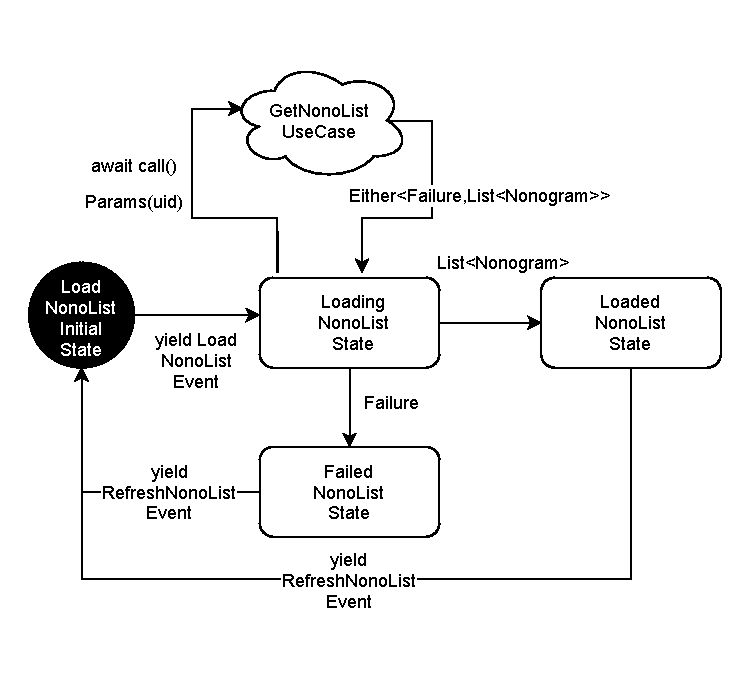
\includegraphics[scale=0.83]{images/statesNonoList.pdf}
  \caption{Diagrama de estado de la funcionalidad Lista de nonogramas en línea}
  \label{fig:nonolist-states}
\end{figure}

Cuando el usuario accede a la sección de nonogramas en línea se manejará, por defecto, el estado
inicial \textit{LoadNonoListInitialState}, que a su vez, enviará el evento \textit{LoadingNonoListEvent}.

En cuanto se envíe tal evento, se tramitará el estado \textit{LoadingNonoListState}, mostrando
un widget de carga.

Durante este estado de ``carga'' pedirá al caso de uso \textit{GetNonoListUseCase} la lista de \textit{nonogramas}
disponible en \textit{Firebase}. Tras esta llamada del caso de uso, nos puede devolver los siguientes
tipos de objeto:

\begin{itemize}
  \item[$\bullet$] La totalidad de \textit{nonogramas} publicados por la comunidad disponible en \textit{Firebase}.
  \item[$\bullet$] Un objeto de tipo \textit{Failure}, indicando que no se ha podido tramitar la operación 
  debido a por ejemplo un error de conexión o de base de datos.
\end{itemize}

En el caso de devolver la lista de \textit{nonogramas} actualizado con éxito, se manejará el estado
\textit{LoadedNonoListState}, mostrando la lista de \textit{rompecabezas} al usuario y en su defecto el estado 
de \textit{FailedNonoListState}, cargando una vista de error. 

El código correspondiente se puede encontrar en
\autoref{cap:anexo1-2}.

\break

\subsection{Desarrollo de la capa de dominio}
El desarrollo de la \textit{capa de dominio} comienza con la definición de casos de uso a usar por el \textit{BLoC}.
Esta implementación se realiza a partir de la clase genérica \textit{usecase} disponible en el paquete \textit{core}.

Como se ha podido comprobar en la \textit{capa de dominio}, este caso de uso devuelve un objeto
de tipo \textit{Either<Failure,Type>}, indicando que puede devolver el tipo de objeto deseado, \textit{Type}, o en caso contrario,
un objeto de tipo \textit{Failure} debido a un error ocurrido en la llamada del repositorio. Adicionalmente, este caso de uso puede
recibir o no una lista de parámetros a usar por el repositorio, como por ejemplo, el \textit{uid} del usuario.

Este aspecto, puede realizarse gracias al paquete externo \textit{dartz}, dotando a \textit{Dart} de aspectos y 
beneficios propios de los lenguajes funcionales.

Una vez definido el caso de uso se definirán las clases genéricas de \textit{repositorios} y \textit{entities} a usar en la
\textit{capa de datos}.

Siguiendo la funcionalidad de \textit{Lista de nonogramas en línea} se puede mostrar la implementación de su \textit{capa 
de dominio} en el \autoref{cap:anexo1-3}.

\subsection{Desarrollo de la capa de datos}
El último paso consiste en desarrollar la \textit{capa de datos} de la funcionalidad, comenzará con la definición de los
\textit{modelos} y la \textit{implementación de los repositorios} a partir de las clases genéricas de \textit{entities} y
\textit{repositories} respectivamente, definidas previamente en la \textit{capa de dominio}.

La implementación de estos \textit{repositorios} emplearán clases de tipo \textit{datasource} que establecerán una conexión
con fuentes de datos externas propias del aplicativo como: i) la base de datos local de la solución y ii) el 
servicio \textit{FireStore} propio de \textit{Firebase}.

Esta \textit{implementación del repositorio} se encargará de
devolver un objeto \textit{Left} o \textit{Right} propio del paquete \textit{dartz}, dependiendo del comportamiento de 
los \textit{datasources} empleados: 

En la funcionalidad citada como ejemplo dichos ejemplos contendrán los siguientes tipos de objeto, tal y como se puede visualizar
en \autoref{cap:anexo1-4}:
\begin{itemize}
  \item[$\bullet$] El objeto \textit{Right} contendrá la lista de nonogramas actualizado obtenido por la llamada a \textit{Firebase} realizada por el 
  \textit{datasource}
  \item[$\bullet$] El objeto \textit{Left} contendrá un \textit{Failure} indicando que no se ha podido tramitar la operación 
  debido a por ejemplo un error de conexión o de base de datos.
\end{itemize}

\subsection{Inyección de dependencias}
Por último, con el fin de ``localizar'' cada una de las capas mencionadas y hacerlas accesibles en cada punto del aplicativo,
se empleará el uso de un \textit{Inyector de dependencias}. 

Esta práctica es altamente recomendable, sobre todo, en soluciones de una
extensión importante. Para ello, se definirá en el directorio \textit{di} del sistema raíz \textit{lib} la clase
\textit{injection\_container.dart}, tal y como se puede visualizar en \autoref{cap:anexo1-5}.

La definición de esta clase se realizará mediante la librería externa \textit{Get\_It}, uno de los \textit{localizadores de servicios}
más popular. En el se crearán \textit{factories} para ``inyectar'' los \textit{BLoCs} y \textit{singletons} para el resto de
servicios (\textit{repositories},\textit{use cases}, \textit{datasources} y servicios externos como \textit{Firebase} y \textit{Sqflite}).